%%%%%%%%%%%%%%%%%%%%%%%%%%%%%%%%%%%%%%%%%

%----------------------------------------------------------------------------------------
%	PACKAGES AND OTHER DOCUMENT CONFIGURATIONS
%----------------------------------------------------------------------------------------

\documentclass{article}

\input{C:/Code/TexStudio/templates/structure.tex} % Include the file specifying the document structure and custom commands

%----------------------------------------------------------------------------------------
%	ASSIGNMENT INFORMATION
%----------------------------------------------------------------------------------------

\title{Assignment \#1} % Title of the assignment

\author{Name:Cao Mingming\\ Student ID:2018311770\\ \texttt{cmm18@mails.tsinghua.edu.cn}} % Author name and email address

\date{Tsinghua University --- \today} % University, school and/or department name(s) and a date

%----------------------------------------------------------------------------------------

\begin{document}

\maketitle % Print the title

\section{Solution 1}

Take $\mu(x,y,z)=\psi(x,y,z)e^{-ikz}$ into the wave equation $\triangledown^2\mu+k^2u=0$, 

\begin{equation}\label{eq1}
 \triangledown _t^2 (\psi e^{-ikz})+\dfrac{\partial^2}{\partial z^2}(\psi e^{-ikz})+k^2\psi e^{-ikz}=0
\end{equation}
where 
$$
\triangledown_t^2=(\dfrac{\partial^2}{\partial x^2}+\dfrac{\partial^2}{\partial y^2})
$$
Expand $\dfrac{\partial^2}{\partial z^2}(\psi e^{-ikz})$ we can get,

\begin{equation}\label{eq2}
\dfrac{\partial^2}{\partial z^2}(\psi e^{-ikz})=(\dfrac{\partial^2 \psi}{\partial z^2}-2ik\dfrac{\partial \psi}{\partial z}-k^2\psi)e^{-ikz}
\end{equation}
Take equation \ref{eq2} into equation \ref{eq1},

\begin{equation}\label{eq3}
 \triangledown _t^2 \psi+\dfrac{\partial^2 \psi}{\partial z^2}-2ik\dfrac{\partial \psi}{\partial z}=0
\end{equation}
In order for paraxial condition to be satisfied, which means $\psi(x,y,z)$ must vary much more slowly along the z-axis than it does along the x- and y-axes.Thus, when substituting
equation\ref{eq2} into the wave equation, $\partial^2\psi/\ \partial z^2$ can be ignored compared to the other second derivatives. So we can rewrite equation \ref{eq1} as

\begin{equation}\label{eq4}
\triangledown_t^2\psi-2ik\dfrac{\partial \psi}{\partial z}=0
\end{equation}
Take the trial function as,
\begin{equation}\label{eq5}
\psi(x,y,z)=exp\{-i(P(z)+\dfrac{k}{2q(z)}r^2)\},r^2=x^2+y^2
\end{equation}
and in the cylindrical coordinate $\triangledown_t^2=\dfrac{\partial^2}{\partial r^2}+\dfrac{1}{r} \dfrac{\partial}{\partial r}+\dfrac{1}{r^2}\dfrac{\partial^2}{\partial \theta^2}$ ,substitute equation \ref{eq5} into equation \ref{eq4} and organized by the order of r.
\begin{equation}\label{eq6}
\dfrac{k^2}{q(z)^2}(\dfrac{dq(z)}{dz}-1)r^2-2k(\dfrac{dP(z)}{dz}+\dfrac{i}{q(z)})=0
\end{equation}
Due to that equation \ref{eq6} is always equal to zero no matter how r varies, which indicates the parameter equals to zero, $$\begin{array}{l}
\dfrac{dq(z)}{dz}-1=0 \\
\\
\dfrac{dP(z)}{dz}+\dfrac{i}{q(z)}=0
\end{array}$$
Finally, we can get
\begin{equation}\label{eq7}
\begin{array}{l}
\dfrac{dq(z)}{dz}=1 \\
\\
\dfrac{dP(z)}{dz}=-\dfrac{i}{q(z)}
\end{array}
\end{equation}

\section{Solution 2}
By solving equation \ref{eq7} we could get, $q(z)=q(z_1)+(z_2-z_1)$.Write the complex beam parameter in two real parameters, $R $ and $\omega$,

\begin{equation}\label{eq8}
\dfrac{1}{q}=\dfrac{1}{R}-i\dfrac{\lambda}{n\pi\omega^2}.
\end{equation}
Substitute equation \ref{eq8} into $\mu(x,y,z)$,

\begin{equation}\label{eq9}
\mu(x,y,z)=exp\{-i(P(z)+kz+k\dfrac{r^2}{2R})-\dfrac{r^2}{\omega^2} \},	
\end{equation}
where $k=2n\pi/\lambda$ is used. Now consider about the surface of constant phase which is r-dependence, which means the phase parameter in equation \ref{eq9} is a constant,
\begin{equation}\label{eq10}
z+\dfrac{r^2}{2R}=constant
\end{equation}
and $P(z)$ has been ignore for that it varies much more slowly than other two terms. R can be interpreted as the radius of wavefront by the equation of calculating the curvature under the paraxial approximation $r\ll R$.

\begin{equation}\label{eq11}
\rho=\dfrac{ds}{d\theta}=\dfrac{{(1+f^{'}(x))}^{3/2}}{f^{''}(x)}.
\end{equation}
Substitute $$z=f(r)=constant-\dfrac{r^2}{2R},$$into equation \ref{eq11},
\begin{equation}\label{eq12}
\rho=R(1+\dfrac{r}{R})^{3/2}
\end{equation}
So the curvature of wave front $\rho=R$ under the paraxial condition $r\ll R$.
Now consider the minimum size of the spot when the wave front becomes a plan ($R=\infty$), the corresponding value of q is:
\begin{equation}\label{eq13}
\text{At waist:}\indent q\equiv q_0=i\dfrac{n\pi\omega^2}{\lambda}
\end{equation}
Setting $z$ as the distance from the waist,$\omega_0$ as the radius of waist, the values of q is,
\begin{equation}\label{eq14}
q(z)=q_0+z=i\dfrac{n\pi\omega^2}{\lambda}+z,
\end{equation}
From equation \ref{eq14} we can derive that,
\begin{equation}\label{eq15}
\begin{array}{l}
\text{Distanace to waist:}\indent d=-Re\{q(z)\}
\\
\\
\text{Rdius of waist:}\indent \omega_0=\sqrt{\dfrac{\lambda}{n\pi}Im\{q(z)\}}
\end{array}
\end{equation}
By solving equation \ref{eq8} and \ref{eq14},we can obtain $\omega$ and $R$ as the function of propagation distance $z$ from waist:
\begin{equation}\label{eq16}
\begin{array}{l}
\omega(z)=\omega_0[1+(\dfrac{\lambda z}{n\pi\omega_0^2})^2]^{1/2}
\\
\\
R(z)=z[1+(\dfrac{n\pi\omega_0^2}{\lambda z})^2].
\end{array}
\end{equation}
The figure of $\omega(z)$ and $R(z)$ is drew as in figure \ref{fig:side:a} and \ref{fig:side:b},where we have assumed that $\omega_0=1,\lambda=1,n=1$ for simplification.

\begin{figure}[h]
	\begin{minipage}[t]{0.5\linewidth}
		\centering
		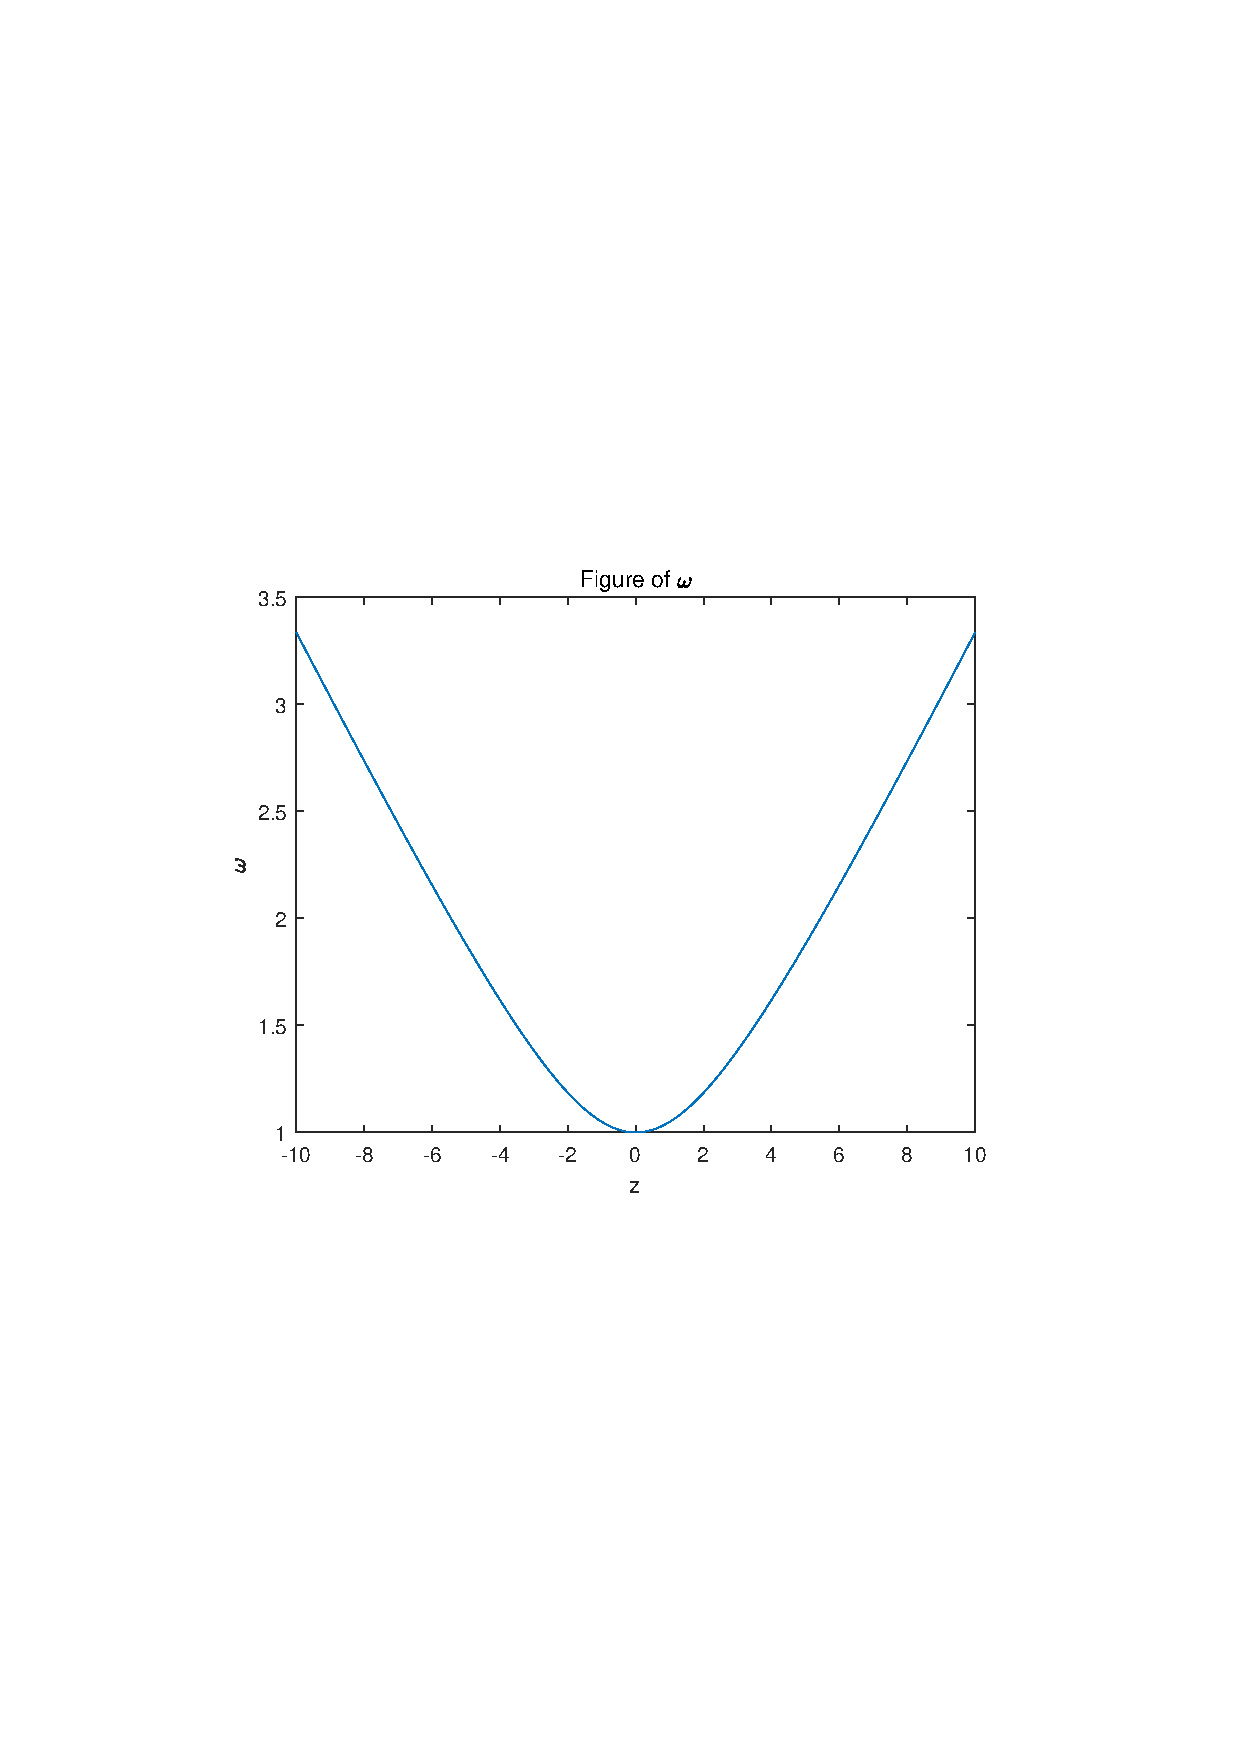
\includegraphics[width=2.2in]{w.pdf}
		\caption{Figure of $\omega(z)$}
		\label{fig:side:a}
	\end{minipage}%
	\begin{minipage}[t]{0.5\linewidth}
		\centering
		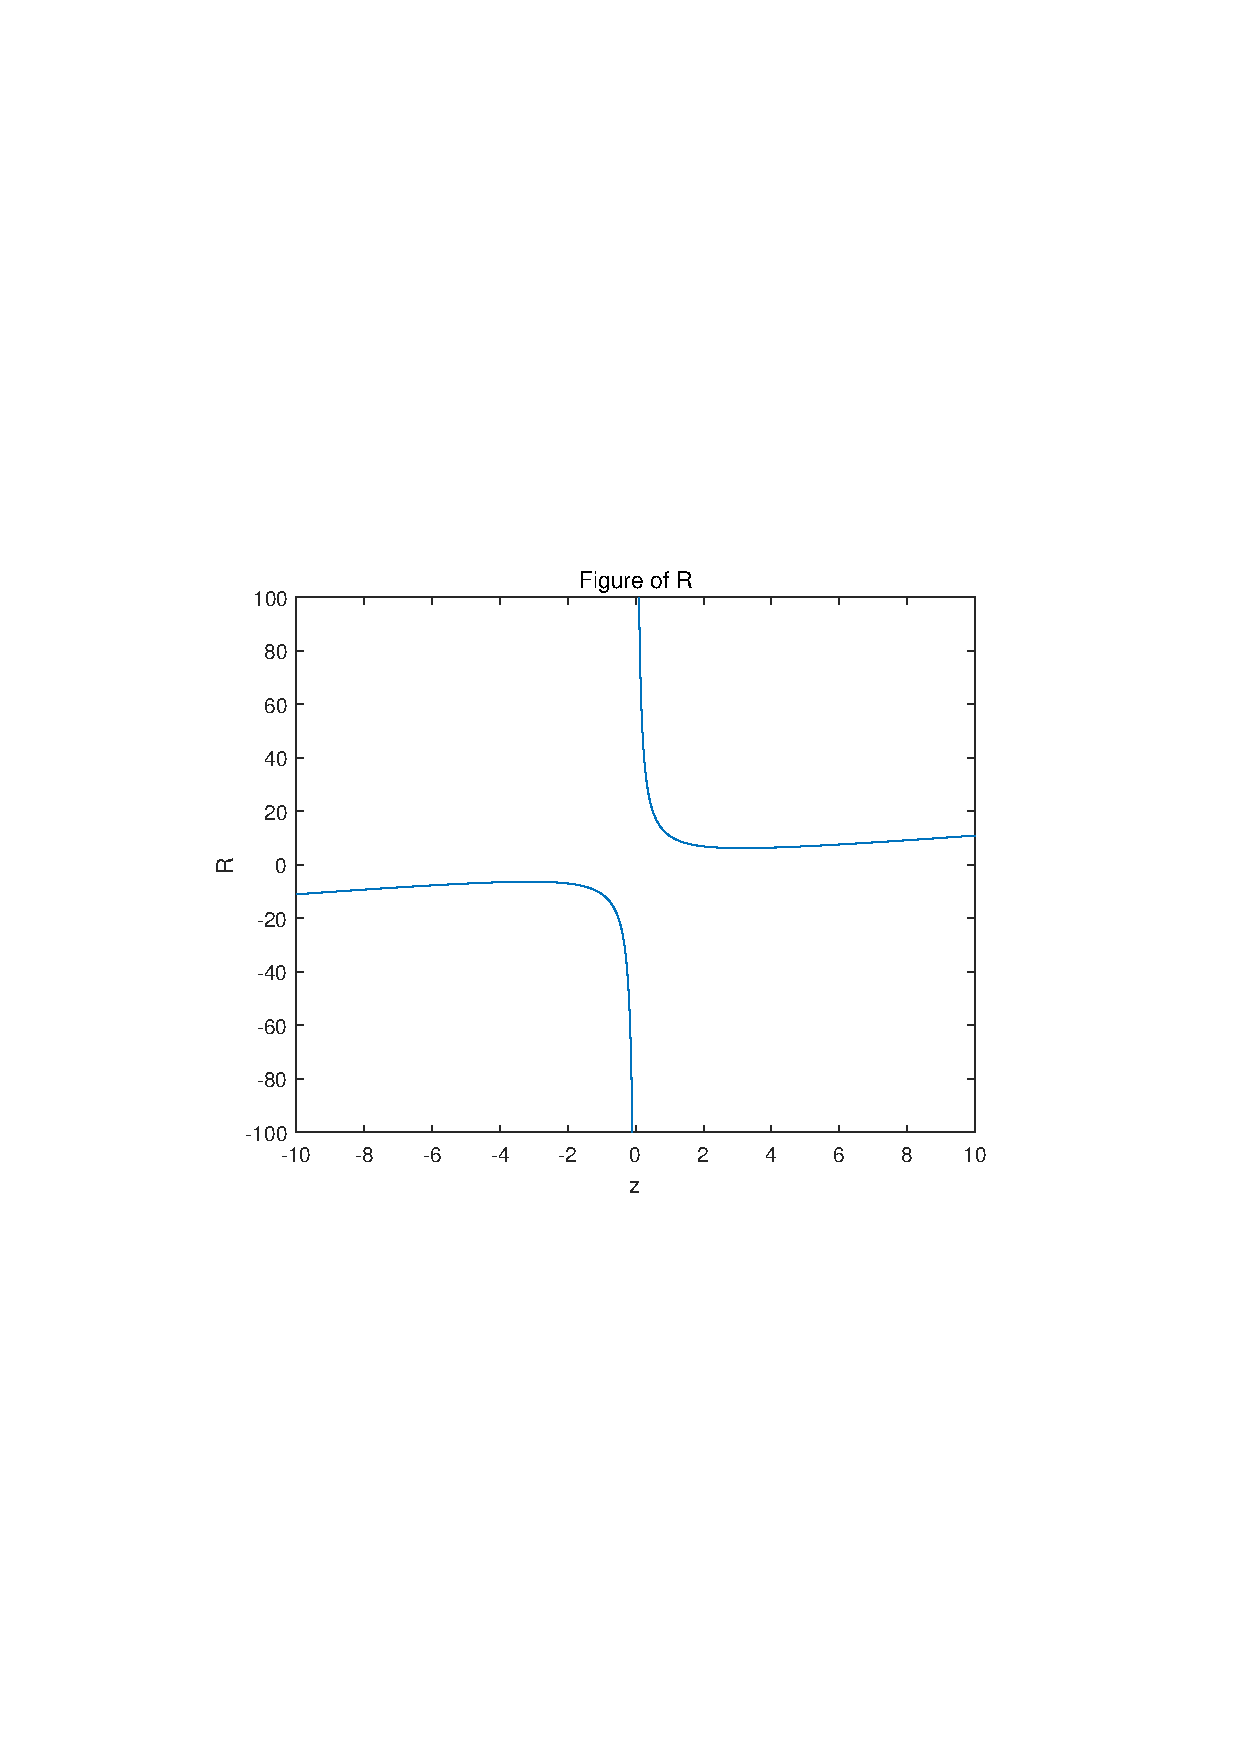
\includegraphics[width=2.2in]{r.pdf}
		\caption{Figure of $R(z)$}
		\label{fig:side:b}
	\end{minipage}
\end{figure}


\end{document}
